% !TEX root = poster.tex
\node [mybox,anchor=north west, font=\fontsize{\fntszL}{\fntszL}\selectfont]
at (\repPos) (boxRep){%
\begin{minipage}{\bxszA}

\bigskip
\bigskip
\bigskip

$x$ are operating conditions, design parameters, various QoIs\\
$\lambda$ are model parameters to be inferred/calibrated
\bigskip
\bigskip
\begin{itemize}
\hrule
\bigskip
\item \color{purple}Default:\color{black} \hspace*{0.5cm}Ignore model errors:

\centerline{
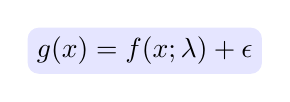
\begin{tikzpicture} \node [rounded corners,fill=blue!10] {
$g(x)=f(x;\lambda)+\epsilon$
};
\end{tikzpicture}
}

\bri
\item Biased or overconfident physical parameters
\item Wrong model predictions
\eri
\bigskip
\bigskip
\hrule
\bigskip
\item  \color{purple}Conventional:\color{black} \hspace*{0.5cm} Correct for model errors:

\bigskip
\centerline{
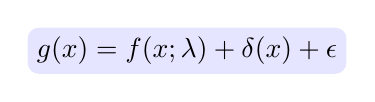
\begin{tikzpicture} \node [rounded corners,fill=blue!10] {
$g(x)=f(x;\lambda)+\delta(x)+\epsilon$};
\end{tikzpicture}
}

\bgi
\item Physical parameters are ok
\egi
\bri
\item Wrong model predictions (data-specific corrections)
\item Model and data errors mixed up
\eri
\bigskip
\bigskip
\hrule
\bigskip
\item  \color{purple}What we do:\color{black} \hspace*{0.5cm} Correct \emph{inside} the model:

\bigskip
\centerline{
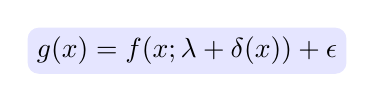
\begin{tikzpicture} \node [rounded corners,fill=blue!10] {
 $g(x)=f(x;\lambda+\delta(x))+\epsilon$};
 \end{tikzpicture}
}

\bgi
\item Embedded model error
\item Preserves model structure and physical constraints
\item Disambiguates model and data errors
\item Allows meaningful extrapolation
\egi
\end{itemize}

\end{minipage}
};
\node[fancytitle, right=10pt, font=\fontsize{\fntszL}{\fntszL}\selectfont]
at (boxRep.north west) {\bf \emph{Embedded} Model Error Representation};
